\subsection{Step responses}
    \subsubsection{First Order System}
        \begin{align*}
            G(s) = \frac{1}{\tau s + 1} \Leftrightarrow 
            \begin{cases*}
                \dot{x} = -\frac{1}{\tau} x + \frac{1}{\tau} u\\
                y = x
            \end{cases*}\\
            \Rightarrow y(t) = 1-e^{-t/\tau}\\
            T_d = \tau \ln(100/d)
        \end{align*}
        \includegraphics[width = \linewidth]{src/images/first_order_step_response.png}
    \subsubsection{Second Order System}
        \begin{align*}
            G(s) = \frac{\omega_n^2}{s^2 + 2 \zeta \omega_n s + \omega_n^2}\\
            \Leftrightarrow 
            \begin{cases*}
                \dot{x} = 
                    \left[\begin{array}{c c}
                        0 & 1\\
                        -\omega_n^2 & -2 \zeta \omega_n
                    \end{array}\right]
                    x + 
                    \left[\begin{array}{c}
                        0\\
                        \omega_n^2
                    \end{array}\right] u\\
                y = x
            \end{cases*}\\
            \Rightarrow y(t) = 1 - \frac{1}{cos(\varphi)}e^{\sigma t} cos(\omega t + \varphi)\\
            T_d = \tau \ln(100/d)\\
            \tau = \frac{1}{|\sigma|}\\
            \text{Time to peak: } T_p = \frac{\pi}{\tau}\\
            \text{Peak overshoot (ratio): } \ln(M_p) = \frac{\sigma \pi}{\omega} = \frac{\zeta \pi}{\sqrt{1 - \zeta^2}} \Rightarrow \zeta^2 = \frac{\ln(M_p)^2}{\pi^2 + \ln(M_p)^2}\\
            \text{Rise time: } T_{100 \%} = \frac{\frac{\pi}{2} - \varphi}{\omega} \approx \frac{\pi}{2 \omega_n}
        \end{align*}
        \titel{Nomenclature}
        \tikzset{
    pattern size/.store in=\mcSize, 
    pattern size = 5pt,
    pattern thickness/.store in=\mcThickness, 
    pattern thickness = 0.3pt,
    pattern radius/.store in=\mcRadius, 
    pattern radius = 1pt}
    \makeatletter
    \pgfutil@ifundefined{pgf@pattern@name@_9395wxxuh}{
    \pgfdeclarepatternformonly[\mcThickness,\mcSize]{_9395wxxuh}
    {\pgfqpoint{-\mcThickness}{-\mcThickness}}
    {\pgfpoint{\mcSize}{\mcSize}}
    {\pgfpoint{\mcSize}{\mcSize}}
    {
    \pgfsetcolor{\tikz@pattern@color}
    \pgfsetlinewidth{\mcThickness}
    \pgfpathmoveto{\pgfpointorigin}
    \pgfpathlineto{\pgfpoint{0}{\mcSize}}
    \pgfusepath{stroke}
}}
\makeatother
% Pattern Info
\tikzset{
    pattern size/.store in=\mcSize, 
    pattern size = 5pt,
    pattern thickness/.store in=\mcThickness, 
    pattern thickness = 0.3pt,
    pattern radius/.store in=\mcRadius, 
    pattern radius = 1pt}
    \makeatletter
    \pgfutil@ifundefined{pgf@pattern@name@_r1aowurqw}{
    \pgfdeclarepatternformonly[\mcThickness,\mcSize]{_r1aowurqw}
    {\pgfqpoint{-\mcThickness}{-\mcThickness}}
    {\pgfpoint{\mcSize}{\mcSize}}
    {\pgfpoint{\mcSize}{\mcSize}}
    {
    \pgfsetcolor{\tikz@pattern@color}
    \pgfsetlinewidth{\mcThickness}
    \pgfpathmoveto{\pgfpointorigin}
    \pgfpathlineto{\pgfpoint{0}{\mcSize}}
    \pgfusepath{stroke}
}}
\makeatother
\tikzset{every picture/.style={line width=0.75pt}} %set default line width to 0.75pt        

\begin{minipage}{0.64\linewidth}
    \def\imgx{175} %\insert linewidth
    \def\imgy{382/618 * \imgx} %golden ratio
    \begin{center} 
        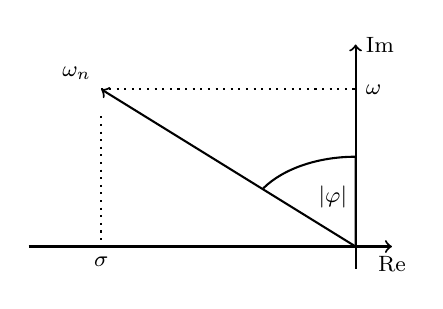
\begin{tikzpicture}[x=0.75pt,y=0.75pt,yscale=-1,xscale=1]            
            %Axis
            %Re
            \draw[->] (0,\imgy*0.9) -- (\imgx,\imgy*0.9);
            \draw (\imgx, 0.9*\imgy) node [anchor = north] [font=\footnotesize] [align=left] {Re};
            %Im
            \draw[->] (\imgx*0.9,\imgy) -- (\imgx*0.9,0);
            \draw (0.9*\imgx, 0) node [anchor = west] [font=\footnotesize] [align=left] {Im};

    
            %Arrow
            \draw [->] (\imgx*0.9, \imgy*0.9) -- (\imgx*0.2, \imgy*0.2); %Arrow \omega_n
            \draw (0.2*\imgx, 0.2*\imgy) node [anchor = south east] [font=\footnotesize] [align=left] {$\omega_n$};

            %Dotted lines
            %\omega
            \draw[dotted] (\imgx*0.2, \imgy*0.2) -- (\imgx*0.9, \imgy*0.2);% \omega
            \draw (0.9*\imgx, 0.2*\imgy) node [anchor = west] [font=\footnotesize] [align=left] {$\omega$};
            %\sigma
            \draw[dotted] (\imgx*0.2, \imgy*0.32) -- (\imgx*0.2, \imgy*0.9);% \sigma
            \draw (0.2*\imgx, 0.9*\imgy) node [anchor = north] [font=\footnotesize] [align=left] {$\sigma$};

    
            %Angle
            \draw (\imgx*0.9,\imgy*0.9) -- (\imgx*0.9,\imgy*0.5) arc
                                    [
                                        start angle=-90,
                                        end angle=-148,
                                        x radius=\imgx*0.3,
                                        y radius=\imgy*0.3
                                    ];
            \draw (0.77*\imgx, 0.68*\imgy) node [anchor = west] [font=\footnotesize] [align=left] {$|\varphi|$};
        \end{tikzpicture}
    \end{center}
\end{minipage}
\begin{minipage}{0.34\linewidth}
    \begin{align*}
        |\omega_n| = \sqrt{\sigma^2 + \omega^2}\\
        |\sigma| = \zeta \omega_n\\
        \varphi = \arctan{\frac{\sigma}{\omega}}\\
        \zeta = \sin(|\varphi|)
    \end{align*}
\end{minipage}
        \includegraphics[width = \linewidth]{src/images/second_order_step_response.png}
